% Options for packages loaded elsewhere
\PassOptionsToPackage{unicode}{hyperref}
\PassOptionsToPackage{hyphens}{url}
\PassOptionsToPackage{dvipsnames,svgnames,x11names}{xcolor}
%
\documentclass[
  authoryear,
  preprint,
  3p]{elsarticle}

\usepackage{amsmath,amssymb}
\usepackage{iftex}
\ifPDFTeX
  \usepackage[T1]{fontenc}
  \usepackage[utf8]{inputenc}
  \usepackage{textcomp} % provide euro and other symbols
\else % if luatex or xetex
  \usepackage{unicode-math}
  \defaultfontfeatures{Scale=MatchLowercase}
  \defaultfontfeatures[\rmfamily]{Ligatures=TeX,Scale=1}
\fi
\usepackage{lmodern}
\ifPDFTeX\else  
    % xetex/luatex font selection
\fi
% Use upquote if available, for straight quotes in verbatim environments
\IfFileExists{upquote.sty}{\usepackage{upquote}}{}
\IfFileExists{microtype.sty}{% use microtype if available
  \usepackage[]{microtype}
  \UseMicrotypeSet[protrusion]{basicmath} % disable protrusion for tt fonts
}{}
\makeatletter
\@ifundefined{KOMAClassName}{% if non-KOMA class
  \IfFileExists{parskip.sty}{%
    \usepackage{parskip}
  }{% else
    \setlength{\parindent}{0pt}
    \setlength{\parskip}{6pt plus 2pt minus 1pt}}
}{% if KOMA class
  \KOMAoptions{parskip=half}}
\makeatother
\usepackage{xcolor}
\setlength{\emergencystretch}{3em} % prevent overfull lines
\setcounter{secnumdepth}{5}
% Make \paragraph and \subparagraph free-standing
\ifx\paragraph\undefined\else
  \let\oldparagraph\paragraph
  \renewcommand{\paragraph}[1]{\oldparagraph{#1}\mbox{}}
\fi
\ifx\subparagraph\undefined\else
  \let\oldsubparagraph\subparagraph
  \renewcommand{\subparagraph}[1]{\oldsubparagraph{#1}\mbox{}}
\fi


\providecommand{\tightlist}{%
  \setlength{\itemsep}{0pt}\setlength{\parskip}{0pt}}\usepackage{longtable,booktabs,array}
\usepackage{calc} % for calculating minipage widths
% Correct order of tables after \paragraph or \subparagraph
\usepackage{etoolbox}
\makeatletter
\patchcmd\longtable{\par}{\if@noskipsec\mbox{}\fi\par}{}{}
\makeatother
% Allow footnotes in longtable head/foot
\IfFileExists{footnotehyper.sty}{\usepackage{footnotehyper}}{\usepackage{footnote}}
\makesavenoteenv{longtable}
\usepackage{graphicx}
\makeatletter
\def\maxwidth{\ifdim\Gin@nat@width>\linewidth\linewidth\else\Gin@nat@width\fi}
\def\maxheight{\ifdim\Gin@nat@height>\textheight\textheight\else\Gin@nat@height\fi}
\makeatother
% Scale images if necessary, so that they will not overflow the page
% margins by default, and it is still possible to overwrite the defaults
% using explicit options in \includegraphics[width, height, ...]{}
\setkeys{Gin}{width=\maxwidth,height=\maxheight,keepaspectratio}
% Set default figure placement to htbp
\makeatletter
\def\fps@figure{htbp}
\makeatother

\makeatletter
\@ifpackageloaded{caption}{}{\usepackage{caption}}
\AtBeginDocument{%
\ifdefined\contentsname
  \renewcommand*\contentsname{Table of contents}
\else
  \newcommand\contentsname{Table of contents}
\fi
\ifdefined\listfigurename
  \renewcommand*\listfigurename{List of Figures}
\else
  \newcommand\listfigurename{List of Figures}
\fi
\ifdefined\listtablename
  \renewcommand*\listtablename{List of Tables}
\else
  \newcommand\listtablename{List of Tables}
\fi
\ifdefined\figurename
  \renewcommand*\figurename{Figure}
\else
  \newcommand\figurename{Figure}
\fi
\ifdefined\tablename
  \renewcommand*\tablename{Table}
\else
  \newcommand\tablename{Table}
\fi
}
\@ifpackageloaded{float}{}{\usepackage{float}}
\floatstyle{ruled}
\@ifundefined{c@chapter}{\newfloat{codelisting}{h}{lop}}{\newfloat{codelisting}{h}{lop}[chapter]}
\floatname{codelisting}{Listing}
\newcommand*\listoflistings{\listof{codelisting}{List of Listings}}
\makeatother
\makeatletter
\makeatother
\makeatletter
\@ifpackageloaded{caption}{}{\usepackage{caption}}
\@ifpackageloaded{subcaption}{}{\usepackage{subcaption}}
\makeatother
\journal{Palaeo3}
\ifLuaTeX
  \usepackage{selnolig}  % disable illegal ligatures
\fi
\usepackage[]{natbib}
\bibliographystyle{elsarticle-harv}
\usepackage{bookmark}

\IfFileExists{xurl.sty}{\usepackage{xurl}}{} % add URL line breaks if available
\urlstyle{same} % disable monospaced font for URLs
\hypersetup{
  pdftitle={Interspecies comparisons of Mg/Ca ratios in limpet shells},
  pdfauthor={Niklas Hausmann; Donna Surge; Francisco Zangrando; Angelica Tivoli; Ivan Briz-Godino},
  pdfkeywords={Sclerochronology, Limpets, Elemental Ratio, Mg/Ca},
  colorlinks=true,
  linkcolor={blue},
  filecolor={Maroon},
  citecolor={Blue},
  urlcolor={Blue},
  pdfcreator={LaTeX via pandoc}}

\setlength{\parindent}{6pt}
\begin{document}

\begin{frontmatter}
\title{Interspecies comparisons of Mg/Ca ratios in limpet shells}
\author[1]{Niklas Hausmann%
\corref{cor1}%
}
 \ead{niklas@palaeo.eu} 
\author[2]{Donna Surge%
%
}

\author[3]{Francisco Zangrando%
%
}

\author[3]{Angelica Tivoli%
%
}

\author[4]{Ivan Briz-Godino%
%
}


\affiliation[1]{organization={Leibniz Zentrum für
Archäologie},addressline={Ludwig-Lindenschmit-Forum
1},city={Mainz},country={Germany},countrysep={,},postcode={55116},postcodesep={}}
\affiliation[2]{organization={University of North
Carolina},addressline={104 South Road, 225 Geology
Building},city={Chapel Hill,
NC},country={US},countrysep={,},postcode={27599-3315},postcodesep={}}
\affiliation[3]{organization={CONICET (Consejo Nacional de
Investigaciones Científicas y Técnicas)},addressline={Avenida Maipú
305},city={Ushuaia},country={Argentina},countrysep={,},postcode={V9410BJA},postcodesep={}}
\affiliation[4]{organization={},country={Spain},countrysep={,},postcodesep={}}

\cortext[cor1]{Corresponding author}





        
\begin{abstract}
This study provides a short reassessment of the use of Magnesium to
Calcium (Mg/Ca) ratios in Atlantic limpet shells to determine past sea
surface temperatures. While \emph{Patella vulgata} along the Spanish
shoreline has since then repeatedly produced reliable correlations
between sea surface temperature and Mg/Ca ratios, this is not the case
for other patelloid species. \emph{Patella vulgata} and \emph{Nacella
deaureata} have been studied using Mg/Ca with mixed or contrary results.
In this study, we present elemental maps of various such species
together with stable oxygen isotope values for some of the specimens.
Our dataset also includes specimens that were previously unsuccessful in
providing significant correlations between δ\textsuperscript{18}O and
Mg/Ca ratios. By reassessing these previous specimens and including a
wider range of modern and archaeological samples from three patelloid
species (\emph{P. vulgata}, \emph{N. deaureata}, and \emph{N.
magellanica}) we further add to the growing set of evidence for the
reliable use of Mg/Ca ratios to detect palaeotemperature change and
serve as a means to determine ontogenetic age and season of capture as
well as to reveal locations of interest within the growth record
(i.e.~annual temperature minima and maxima) for the targeted analysis
using δ\textsuperscript{18}O or clumped oxygen isotope analysis.
\end{abstract}





\begin{keyword}
    Sclerochronology \sep Limpets \sep Elemental Ratio \sep 
    Mg/Ca
\end{keyword}
\end{frontmatter}
    
\section{Introduction}\label{Introduction}

Limpet shells are commonly found within archaeological sites and and
past shorelines due to their robust carbonate structure and the
long-term use of limpets as a marine food source. They have successfully
been studied in the past in the context of coastal subsistence
economies, site occupation on seasonal
\citep{shackleton1973, Parker2018-wf, Bosch2018-ud} or long-term scale
\citep{Ortiz2015-mr}, as well as palaeotemperature
\citep{Fenger2007-gf, Surge2012-ba, Wang2012-ee, Colonese2012-ct, Ferguson2011-zl}.
Determining past sea surface temperature (SST) change largely relies on
the measurement of δ\textsuperscript{18}O-values within the calcitic
parts of the shell, but attempts have been made to also use elemental
ratios, such as magnesium to calcium (Mg/Ca), to have an alternative
measure, that potentially provides a more accurate SST estimate than
δ\textsuperscript{18}O-values, which are also affected by changes in
salinity. In addition, the data acquisition of elemental ratios ---
either through laser-ablation-isotope-ratio-mass-spectrometry
(LA-ICP-MS) or laser induced breakdown spectroscopy (LIBS), can be much
faster and cost-effective, increasing the number of specimens that can
be studied overall \citep{Durham2017-fh, Hausmann2023-ih}.

Problematically, links between Mg/Ca ratios and SST changes in limpets
have also been shown to be unreliable \citep{Graniero2015-zv} and even
where they were successful, anomalous patterns in some specimens had to
be filtered out, reducing the overall robustness of the results of those
successful studies \citep{Ferguson2011-zl}.

While recent research particularly of \emph{Patella} sp. in the
Mediterranean and Southwest Europe have provided promising results
\citep{Hausmann2019-fi, Garcia-Escarzaga2015-jc, Garcia-Escarzaga2018-nf}.
There remains unclarity for Atlantic limpet species, particularly since
it was last shown here, that they are not reliable recorders of
palaeotemperature \citep{Graniero2015-zv}.

In this study we will repeat and expand the analysis of Atlantic limpets
to determine the reliability of Mg/Ca ratios as palaeotemperature
proxies. To do this, we sampled a set of previously published and
unpublished limpet specimens dating to modern and archaeological
contexts using LIBS. LIBS allows us to carry out 2D imaging of entire
shell sections, which helps us to navigate the complex elemental
structure of the shell and better separate the external,
temperature-related changes from the internal and less understood
factors that influence the Mg/Ca ratio.

Relying and adding onto published datasets, allowed us to simultaneously
avoid costs for new high-resolution δ\textsuperscript{18}O-data, use
real-world examples, and also provide pilot-data for areas of existing
research interest. Generally establishing the usefulness and reliabilty
of Mg/Ca as SST proxy in limpets should help to provide a platform for
future research and an important stepping stone to better understand
elemental ratios in other marine mollusc shells.

\section{Materials and Methods}\label{Methods}

\subsection{Limpet specimens}\label{limpet-specimens}

\subsubsection{Modern specimens}\label{modern-specimens}

The analysed specimens, their origin and respective studies with
research background information can be found in Table 1. Here we will
briefly summarise their contextual information, which can be accessed in
more detail at the respective studies
\citep{Nicastro2020-ih, Surge2012-ba, Graniero2017-io}. While those
studies also included other specimens, their accessibility or state of
preservation did not all lend them to be re-analysed.

There are two main locations that we sourced specimens from: the island
of West Ray in Orkney (UK) and the Beagle Channel in Tierra del Fuego
(Argentina). A modern shell on West Ray was collected in Rack Wick Bay
in August 2009, which experiences virtually no freshwater input. The
temperature

\begin{longtable}[]{@{}
  >{\raggedright\arraybackslash}p{(\columnwidth - 10\tabcolsep) * \real{0.1667}}
  >{\raggedright\arraybackslash}p{(\columnwidth - 10\tabcolsep) * \real{0.1667}}
  >{\raggedright\arraybackslash}p{(\columnwidth - 10\tabcolsep) * \real{0.1667}}
  >{\raggedright\arraybackslash}p{(\columnwidth - 10\tabcolsep) * \real{0.1667}}
  >{\raggedright\arraybackslash}p{(\columnwidth - 10\tabcolsep) * \real{0.1667}}
  >{\raggedright\arraybackslash}p{(\columnwidth - 10\tabcolsep) * \real{0.1667}}@{}}
\caption{Table 1 Overview of the modern and archaeological limpet
specimens analysed in this study \{\#tab:specimens\}}\tabularnewline
\toprule\noalign{}
\begin{minipage}[b]{\linewidth}\raggedright
Context
\end{minipage} & \begin{minipage}[b]{\linewidth}\raggedright
Study
\end{minipage} & \begin{minipage}[b]{\linewidth}\raggedright
Species
\end{minipage} & \begin{minipage}[b]{\linewidth}\raggedright
Location
\end{minipage} & \begin{minipage}[b]{\linewidth}\raggedright
Sample ID
\end{minipage} & \begin{minipage}[b]{\linewidth}\raggedright
Previous analyses
\end{minipage} \\
\midrule\noalign{}
\endfirsthead
\toprule\noalign{}
\begin{minipage}[b]{\linewidth}\raggedright
Context
\end{minipage} & \begin{minipage}[b]{\linewidth}\raggedright
Study
\end{minipage} & \begin{minipage}[b]{\linewidth}\raggedright
Species
\end{minipage} & \begin{minipage}[b]{\linewidth}\raggedright
Location
\end{minipage} & \begin{minipage}[b]{\linewidth}\raggedright
Sample ID
\end{minipage} & \begin{minipage}[b]{\linewidth}\raggedright
Previous analyses
\end{minipage} \\
\midrule\noalign{}
\endhead
\bottomrule\noalign{}
\endlastfoot
Modern & \citep{Nicastro2020-ih} & \emph{N. deaureata} & Cambaceres Bay
- Tierra del Fuego (AR) & ND-1016-3 & Stable oxygen and carbon isotope
analysis \\
& & & & ND-1016-4 & \\
& & \emph{N. magellanica} & & NM-1016-1 & \\
& & & & NM-1016-3 & \\
& \citep{Graniero2017-io} & \emph{P. vulgata} & Rack Wick Bay - Westray
(UK) & ORK-LT5 & Stable oxygen and carbon isotope analysis; Mg, Li, Sr,
Ca,. \\
Archaeological & \citep{Surge2012-ba} & \emph{P. vulgata} & Rack Wick
Bay - Westray (UK) & QG1-7188-1 & Stable oxygen and carbon isotope
analysis \\
& & & & QG1-7189-2 & \\
& & & & QG2-1061-1 & \\
& & & & QG2-1064-1 & \\
& & & & QG2-7180-1 & \\
& & & & QG2-7180-2 & \\
& & & & QG1-7246-1 & \\
& This study & \emph{N. magellanica} & Heshkaia 35 in Moat Bay - Tierra
del Fuego (AR) & Heshkaia\_35-1 & \emph{none} \\
& & \emph{N. deaureata} & & Heshkaia\_35-2 & \\
& & \emph{N. deaureata} & & Heshkaia\_35-3 & \\
& & \emph{N. magellanica} & & Heshkaia\_35-4 & \\
& & \emph{N. magellanica} & & Heshkaia\_35-5 & \\
& & \emph{N. magellanica} & & Heshkaia\_35-6 & \\
& & \emph{N. magellanica} & & Heshkaia\_35-7 & \\
& & \emph{N. deaureata} & & Heshkaia\_35-8 & \\
& & \emph{N. magellanica} & & Heshkaia\_35-9 & \\
\end{longtable}

\begin{figure}[H]

{\centering 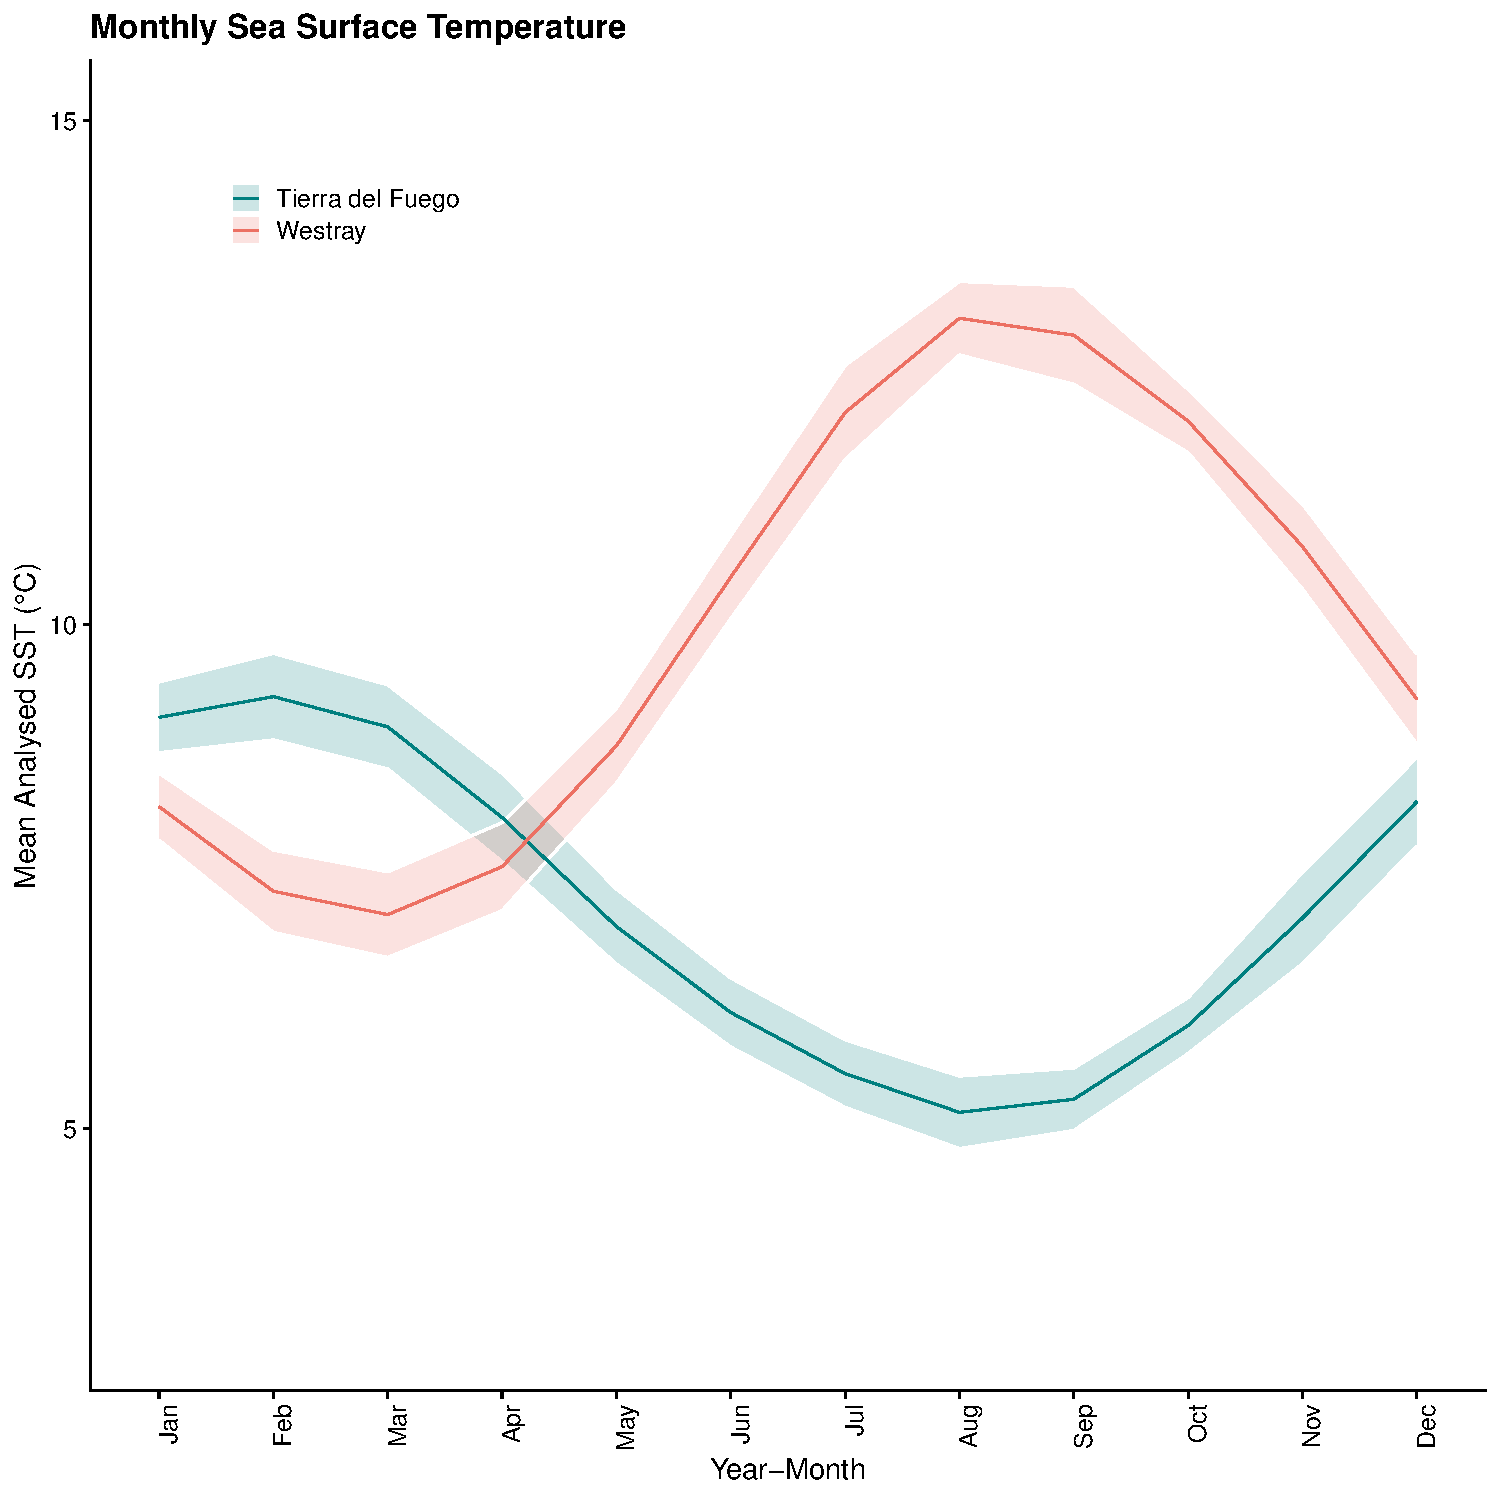
\includegraphics{Manuscript_files/figure-pdf/SST Data-1.pdf}

}

\caption{SST values averaged over the last 20 years. SST values were
sourced from \citep{europeanunion-copernicusmarineservice2015}}

\end{figure}%

\subsubsection{Archaeological specimens}\label{archaeological-specimens}

\subsection{Oxygen isotopes}\label{oxygen-isotopes}

\subsection{Mg/Ca ratios}\label{mgca-ratios}

\section{Results}\label{Results}

\subsection{Patella vulgata}\label{patella-vulgata}

\subsection{Nacella deaureata}\label{nacella-deaureata}

\subsection{Nacella magellanica}\label{nacella-magellanica}

\section{}\label{section}

\begin{figure}[H]

{\centering 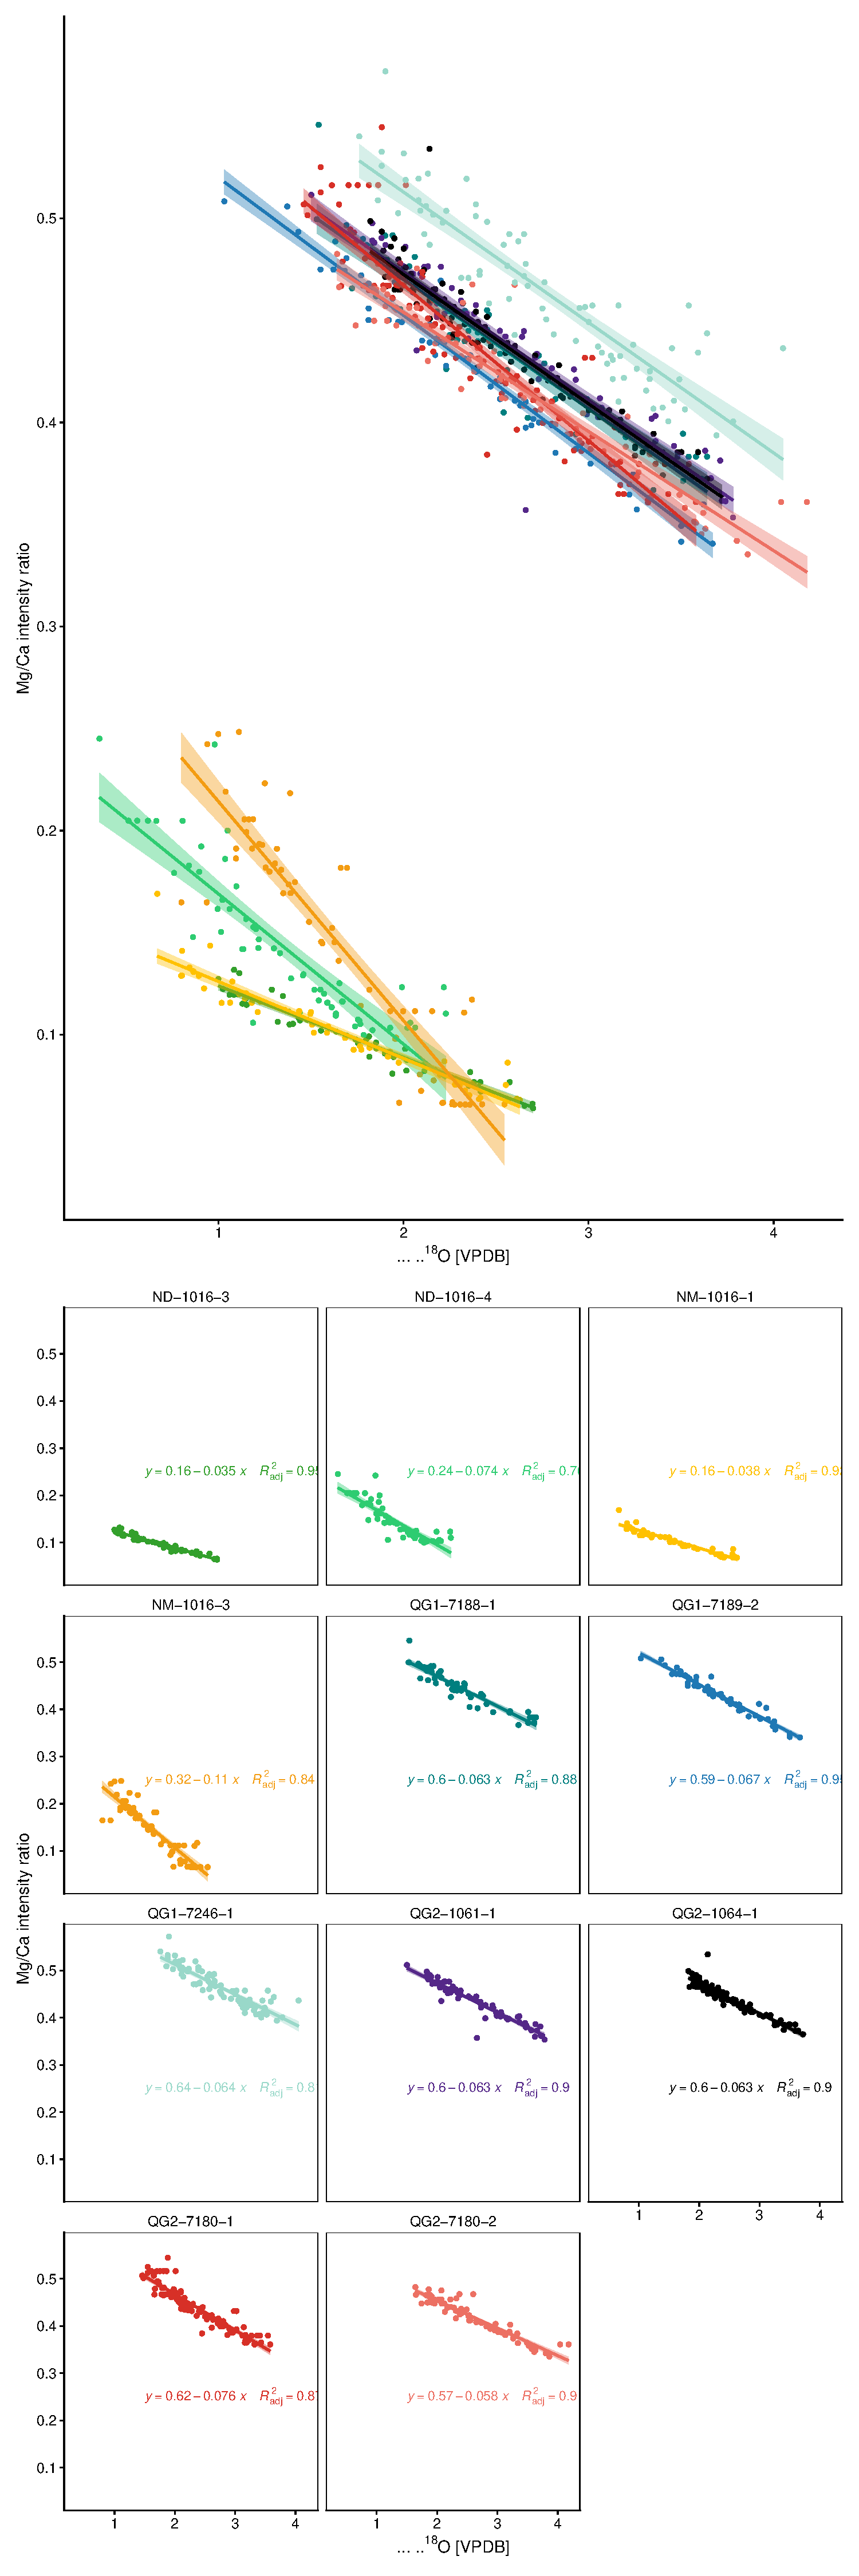
\includegraphics{Manuscript_files/figure-pdf/Correlation Graphs-1.pdf}

}

\caption{Correlation graphs for all specimens}

\end{figure}%

\section{Discussion}\label{discussion}

\subsection{Other correlations}\label{other-correlations}

\begin{figure}[H]

{\centering 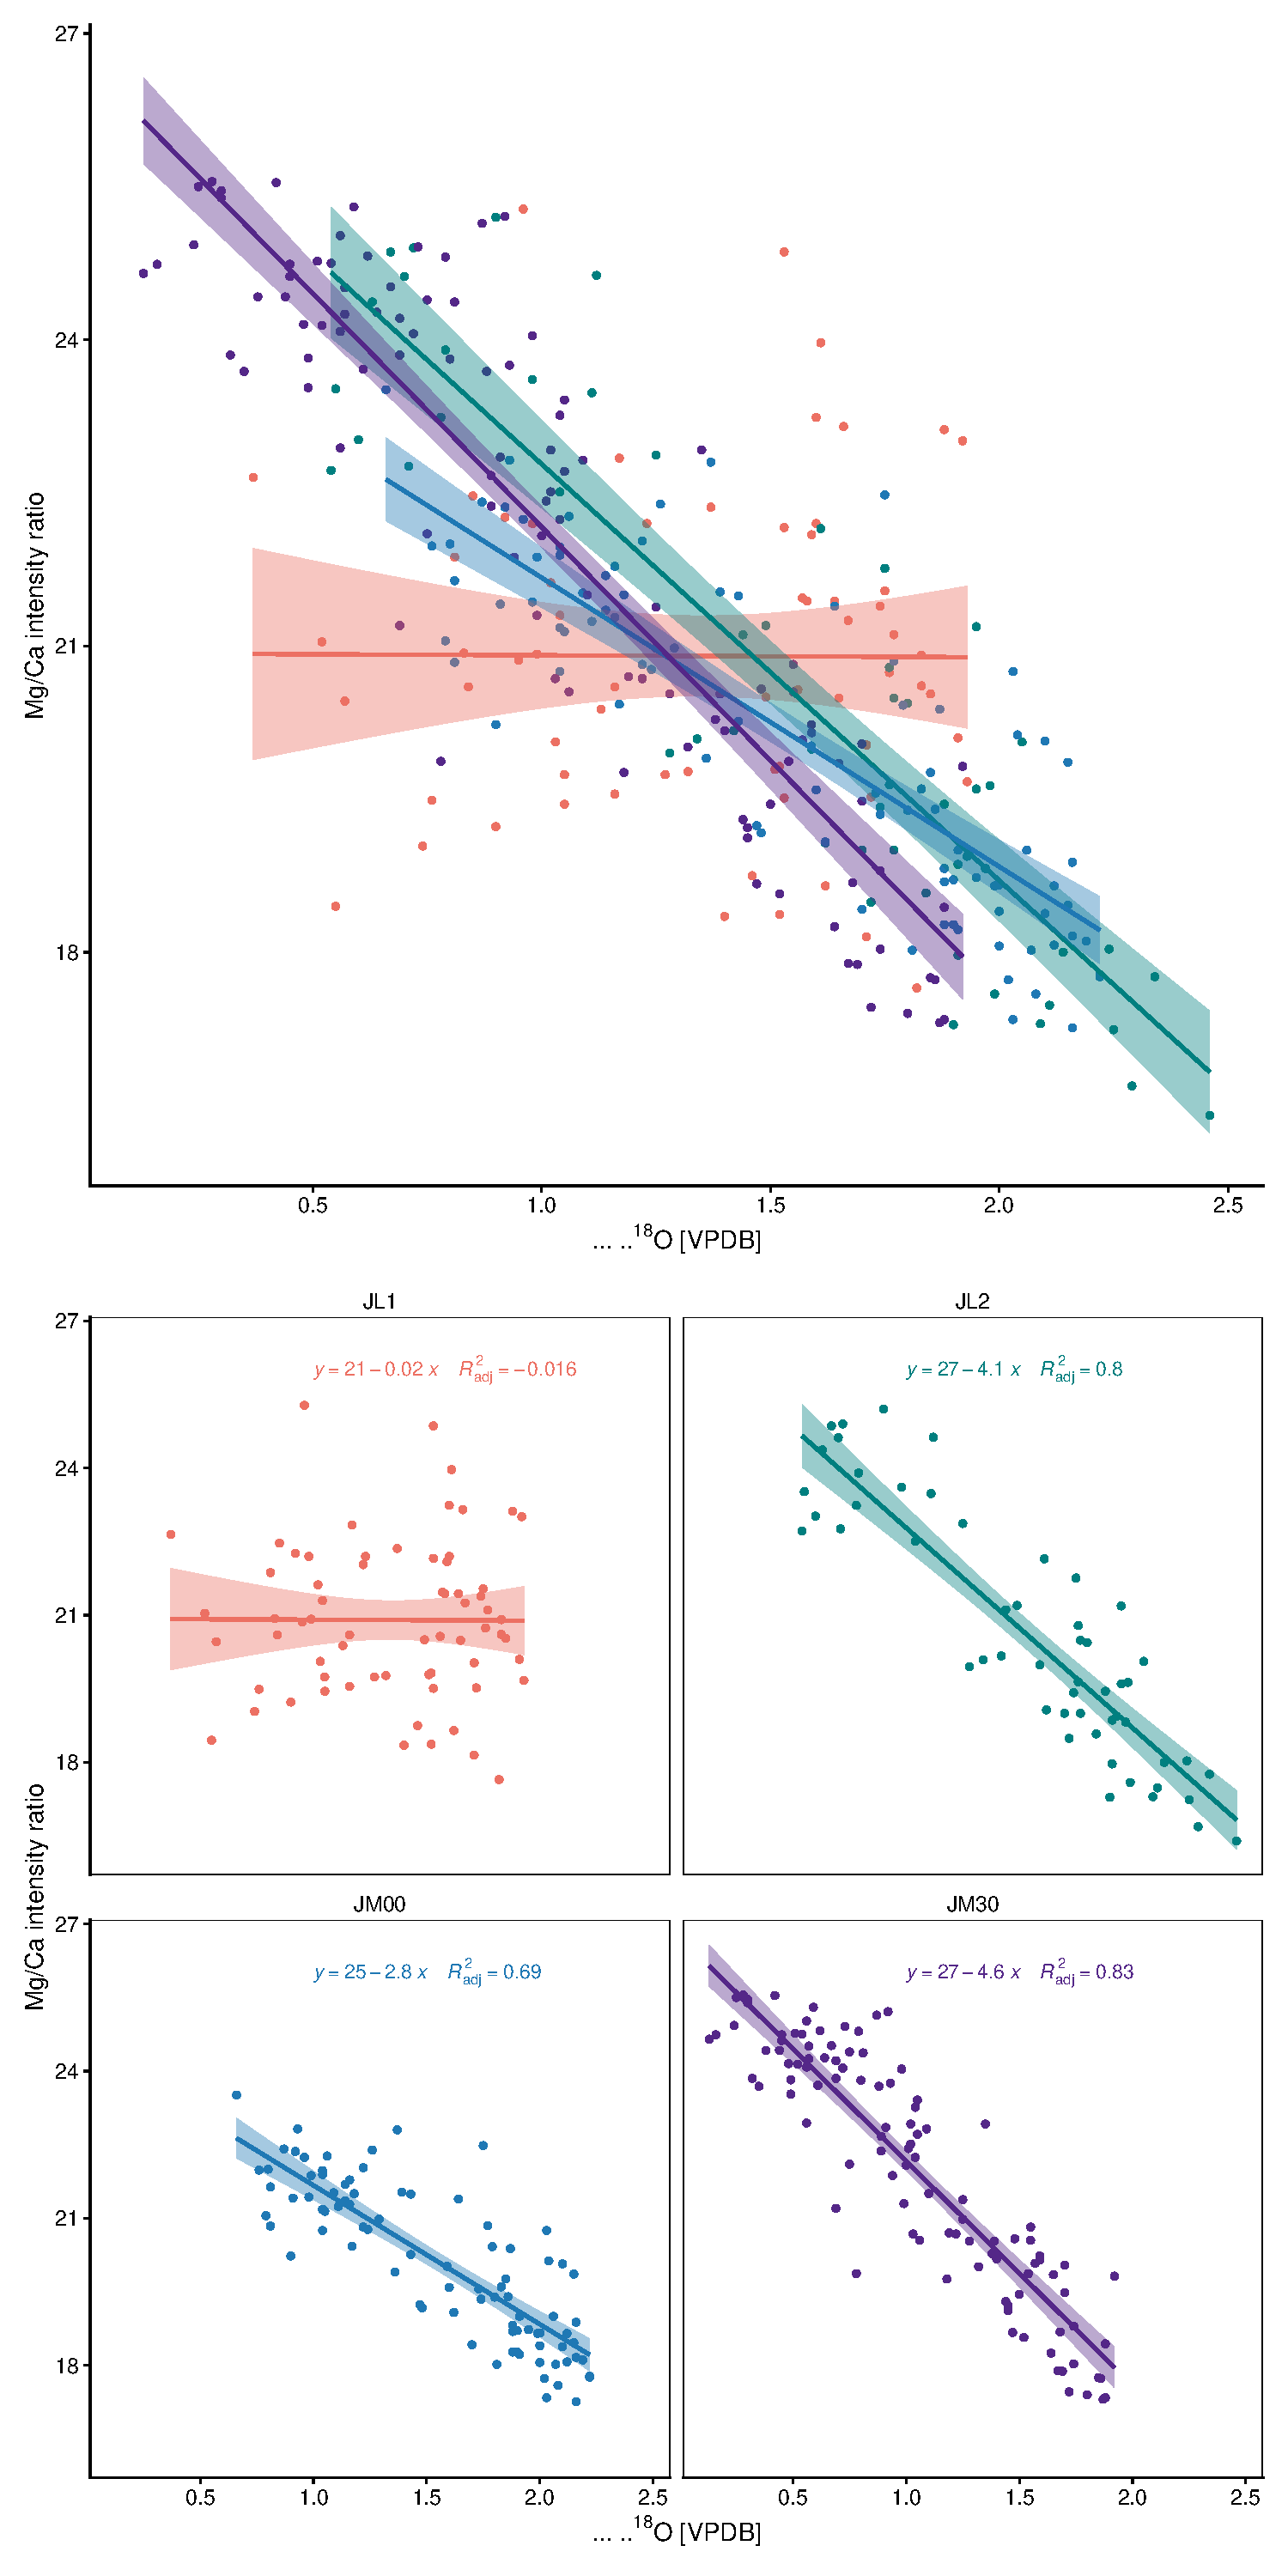
\includegraphics{Manuscript_files/figure-pdf/Ferguson Data-1.pdf}

}

\caption{Correlation graphs for Ferguson et al.~specimens}

\end{figure}%

\begin{longtable}[]{@{}
  >{\raggedright\arraybackslash}p{(\columnwidth - 8\tabcolsep) * \real{0.2000}}
  >{\raggedright\arraybackslash}p{(\columnwidth - 8\tabcolsep) * \real{0.2000}}
  >{\raggedright\arraybackslash}p{(\columnwidth - 8\tabcolsep) * \real{0.2000}}
  >{\raggedright\arraybackslash}p{(\columnwidth - 8\tabcolsep) * \real{0.2000}}
  >{\raggedright\arraybackslash}p{(\columnwidth - 8\tabcolsep) * \real{0.2000}}@{}}
\caption{Table 2: Overview of comparative correlations
\{\#tab:correlations\}}\tabularnewline
\toprule\noalign{}
\begin{minipage}[b]{\linewidth}\raggedright
Species
\end{minipage} & \begin{minipage}[b]{\linewidth}\raggedright
Locality
\end{minipage} & \begin{minipage}[b]{\linewidth}\raggedright
Specimen
\end{minipage} & \begin{minipage}[b]{\linewidth}\raggedright
Correlation R\textsuperscript{2}
\end{minipage} & \begin{minipage}[b]{\linewidth}\raggedright
Study
\end{minipage} \\
\midrule\noalign{}
\endfirsthead
\toprule\noalign{}
\begin{minipage}[b]{\linewidth}\raggedright
Species
\end{minipage} & \begin{minipage}[b]{\linewidth}\raggedright
Locality
\end{minipage} & \begin{minipage}[b]{\linewidth}\raggedright
Specimen
\end{minipage} & \begin{minipage}[b]{\linewidth}\raggedright
Correlation R\textsuperscript{2}
\end{minipage} & \begin{minipage}[b]{\linewidth}\raggedright
Study
\end{minipage} \\
\midrule\noalign{}
\endhead
\bottomrule\noalign{}
\endlastfoot
\emph{P. depressa} & Northern Spain & LAN541 & 0.87 &
\citep{garcía-escárzaga2021} \\
& & LAN545 & 0.86 & \\
& & LAN554 & 0.78 & \\
& & LAN559 & 0.82 & \\
\emph{P. caerulea} & Croatia & ISTPC1 & 0.9 & \citep{Hausmann2019-fi} \\
& & ISTPC2 & 0.84 & \\
& Crete & AF1911A & 0.91\footnote{SST only, no other geochemical data
  available} & \\
& & AF3003A & 0.92\footnote{SST only, no geochemical data available}
& \\
& Israel & AKKPC2 & 0.96 & \\
& & AKKPC3 & 0.89 & \\
& & FRMPC1 & 0.84 & \\
& & FRMPC2 & 0.96 & \\
& Libya & MO31A & 0.83 & \\
& & MP64A & 0.33 & \\
& & MP67A & 0.96 & \\
& & MP68A & 0.81 & \\
& Malta & MA10 & 0.82 & \\
& Tunisia & TUNPC1 & 0.81 & \\
& & TUNPC2 & 0.78 & \\
& Turkey & ANTPC1 & 0.95 & \\
& & ANTPC2 & 0.93 & \\
& & KIZPC1 & 0.94 & \\
& & KIZPC2 & 0.86 & \\
\emph{P. rustica} & Gibraltar & JL1 & 0.02 & \citep{Ferguson2011-zl} \\
& & JL2 & 0.8 (0.79) & \\
\emph{P. caerulea} & Gibraltar & JM00 & 0.69 (0.79) & \\
& & JM30 & 0.83 (0.79) & \\
\emph{P. vulgata} & Orkney & ORK-LT5 & not reported, here 0.88 &
\citep{Graniero2017-io} and this study \\
& & & & \\
& & & & \\
& & & & \\
\end{longtable}

\subsection{Comparison of ORK-LT5}\label{comparison-of-ork-lt5}

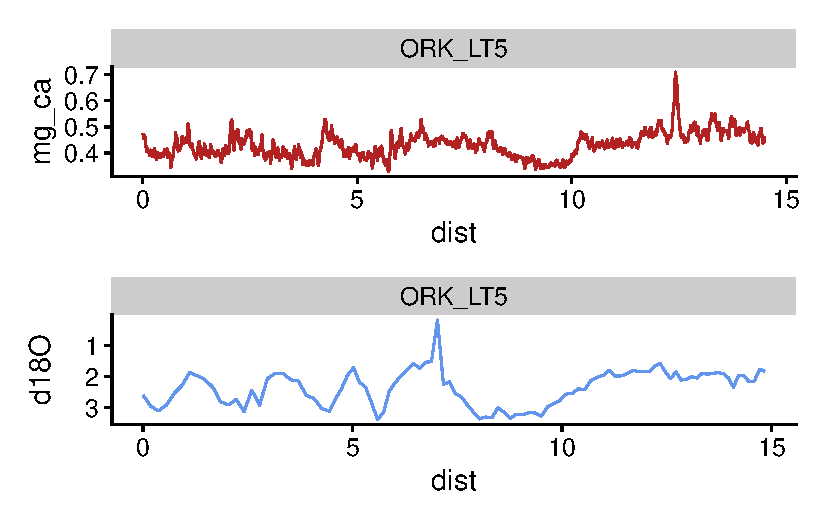
\includegraphics{Manuscript_files/figure-pdf/unnamed-chunk-1-1.pdf}

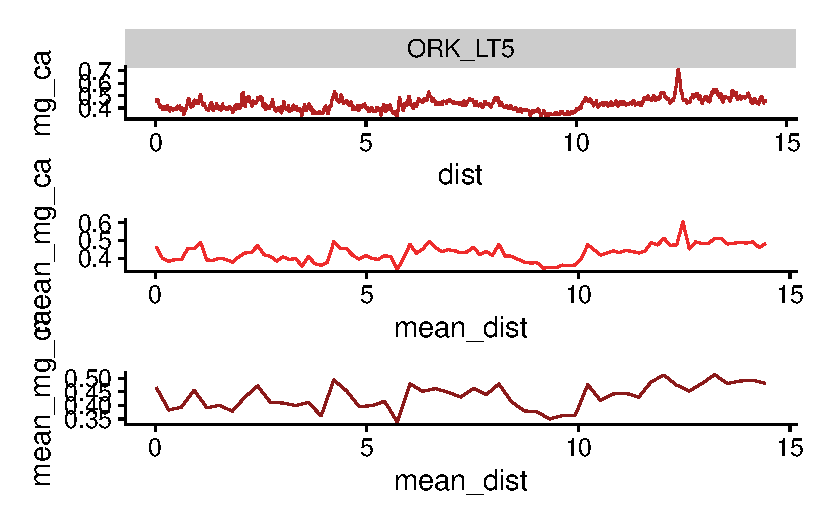
\includegraphics{Manuscript_files/figure-pdf/subsample-1.pdf}


  \bibliography{bibliography.bib}


\end{document}
